%# -*- coding: utf-8-unix -*-
%%==================================================
%% chapter04.tex for SJTU Bachelor Thesis
%%==================================================

%\bibliographystyle{sjtu2}%[此处用于每章都生产参考文献]
\chapter{基于集群仿真的调度器设计与优化}
虽然在直觉上,基于巨型虚拟机的调度器可提高集群的CPU使用率,但目前我们无法在大型集群上验证我们的实现,同时在大型集群上验证的耗时过长,不易及时发现调度器的性能瓶颈并且快速调整相关参数。本章利用谷歌提供的大型集群中任务调度与任务资源使用情况的追踪数据(trace data)模拟大型集群中真是的任务负载,对之前提出的调度策略进行仿真,并优化其调度算法。在开始使用追踪数据之前,应当对追踪数据的内容有大致了解。

\section{集群追踪数据简述}
本文使用的集群追踪数据来自于谷歌的Borg集群(称为cell),包含了一个含有12.5k台机器的集群在29天的追踪周期里的运行情况。具体来说,我们用于集群仿真的数据是ClusterData-2011-2,从北美东部夏令时2011年五月一日的19点整开始进行追踪,持续了29天。较长的追踪时间和较大的机器数量保证了追踪数据的代表性和说服力,能够真实地反应分布式集群的任务负载及其调度情况。Borg\cite{borg}是谷歌在2015年提出的分布式集群调度框架,对于一个Borg集群(称为cell),有一个对应的Borg Master,而每个节点上运行一个Borglet,与Borg Master通信,作出资源分配决策。Borglet计算任务负载并将计算结果放在缓存中,并与Borg Master沟通需要进行的操作,但不与Borg Master频繁沟通,为了防止Borg Master负载过重而宕机。Borg使用容器做到了资源的细粒度分配与限制,资源用量数据通过容器来测量。追踪数据分为对以下几个方面的数据的记录:机器事件(机器加入或离开集群,以及配置更新)、机器属性(包含对机器内核版本、硬件配置、网络配置等多个属性),以及作业(Job)和任务(Task)事件表,记录了作业和任务的生命周期,以及任务在各个采样时间段的资源用量情况。在任何一组数据中,都含有一个或几个时间戳。追踪数据中的时间戳是一个64位的无符号整数,从追踪时间段的前600秒算起,这是为了支持两个特殊时间戳:0代表发生在追踪时间段之前的事件,而$2^{64}-1$(最大的64位无符号数)表示发生在追踪时间段之后的事件。丰富的数据类型对集群的工作状态进行了详细的描述,利用这些数据可以完整地复现一个真实大小的集群,相比于在真实集群上进行测试,可以相当快速地完成模拟。

本文主要使用追踪数据中的两组数据来模拟不同的调度策略:$task\_usage$,每个采样时刻的任务资源用量数据和$task\_event$,任务调度状态变更事件数据。在每一条$task\_usage$数据是各个采样间隔的任务资源用量数据,需要关注的字段有:(1)采样时间段的起始时间和终止时间,(2)任务号,进程号,用于标识一个唯一的进程。(3)平均CPU使用率,最大CPU使用率,(4)用户可访问的内存页数目、最大用户可访问内存页数目、分配给整个容器进程的内存页数目(包括部分用户不可访问的内核页面)。这些数据都是通过测量容器的内存占用量获得的。(5)performance counter相关数据,CPI是平均每条指令花费的CPU周期数,MPI是平均每条指令访问内存的次数。注意,所有资源用量数据均是对最大值标准化过的,例如,所有进程的CPU使用量是1,2,3,4,则在数据中是1/4,2/4,3/4,4/4。在每一条$task\_event$数据是任务事件(包括$SUBMIT$、$SCHEDULE$、$EVICT$、$FAIL$、$FINISH$等)的列表,需要关注的字段有:(1)任务事件发生的时间戳,记录了该任务事件发生的时间点。(2)任务号,进程号,用于标识一个唯一的进程。(3)任务优先级。在追踪数据中,任务的优先级最高为11,最低为0,优先级高的进程可以抢占优先级低的进程的资源。其中几个特殊的优先级有:空闲优先级(0-1),这是最低的优先级,基本不要求资源;产品优先级(9-11),是集群中最高的优先级,调度器避免这个优先级的进程资源被挤占;监控优先级(12),用于监控其他任务的健康状况。(4)CPU、内存资源请求量:进程使用资源的上限,超过这个限制的进程会被限制或杀死。(5)事件类型:标识了进程生命周期中的事件类型。主要的进程事件有:(1)$SUBMIT$:进入$PENDING$状态,进程有资格被调度运行;(2)$SCHEDULE$:进程被调度运行进入$RUNNING$状态,开始真正的占用系统资源(3)$FINISH$:进程正常退出,由$RUNNING$状态变为$DEAD$状态。

\section{粗粒度调度器的仿真}
做集群模拟之前,需要做一些简化假设:
\begin{itemize}
  \item 假设任何一个被$SUBMIT$的进程都将被调度到任意的节点上,集群中除了巨型虚拟机中的调度器外再无集群调度器;
  \item 集群中的机器数量在运行过程中没有变化,没有机器宕机也没有新机器加入集群,每个机器的处理能力也不随时间变化
  \item 网络开销仅计算进程迁移时进程所拥有的内存页(本文选取分配给整个容器进程的内存页)迁移造成的开销;
  \item 网络数据传输不耗费时间,且网络状态始终保持良好,不会出现network partition(网络分割),没有网络带宽的限制。
  \item 假设巨型虚拟机运行不占用节点上的资源,dQEMU进程和DSM不占用CPU和内存。
\end{itemize}

\subsection{仿真系统的建立}
在上述假设成立的条件下,我们用python脚本(simulator.py)模块化地设计如下仿真系统:
\begin{figure}
\centering
\begin{minipage}[c]{0.62\textwidth}
\begin{lstlisting}[language=python]
class Task:
    def __init__(self, task_id, duration,
        priority, request, usage):
        self.running_start, self.schedule = 0, 0
        self.duration = duration
        self.priority = priority
        self.request = request
        self.usage = usage
\end{lstlisting}
\end{minipage}
\begin{minipage}[c]{0.5\textwidth}
\begin{lstlisting}[language=python]
class Machine:
    def __init__(self, machine_id):
        self.machine_id = machine_id
        self.tasks = set()
        self.tasks_completion = []
        self.pending = set()
        self.request = 0.0
\end{lstlisting}
\end{minipage}
\begin{minipage}[c]{0.8\textwidth}

\begin{lstlisting}[language=python]
class Scheduler:
    def __init__(self):
        self.machines,self.average = [],[]
        self.gini, self.exceeded_load = [], []
        self.machines=[Machine(i) for i in range(n_machines)]
        self.migration_mem = 0.0
\end{lstlisting}
\end{minipage}
\end{figure}

\noindent\textbf{进程类(Task)}\quad \label{chap:task}进程类表示一个可以被集群调度的实体,占用集群资源。进程类中的字段有:每个进程的进程号,优先级,CPU使用率上限,和一些时间戳,包括被调度的时刻$schedule$),开始运行的时刻$running\_start$,以及在资源没有被挤兑或抢占时应该获得的运行时间$duration$,还有每个追踪时间段的资源用量列表(包括平均CPU使用率,最大CPU使用率,以及分配给整个容器进程的)。在读取$task\_event$数据时,将$SUBMIT$事件的时间戳填入到Task类的$schedule$字段中,表示进程被调度到某个机器上(不一定开始运行);将$SCHEDULE$到$FINISH$的时间差填入$duration$字段,表示进程以最充足资源完成所消耗的时间;将CPU使用率上限填入$request$字段。在读取$task\_usage$数据时,将$usage$字段用每个追踪时间段的资源用量列表填满。由于我们没有考虑$EVICT$事件,所以当Machine类中被调度运行的任务的负载总和超过了其真实负载时,我们将该Machine类中所有的Task的$duration$字段在每个时钟周期中加上一个值(见后文介绍)。于是,我们可以通过Task的$duration$字段与等待被调度运行的时间之和($duration + schedule - running\_start$)判断QoS violation的程度(称作$duration$),即服务质量的影响程度。$duration$表征了一个任务从被调度到运行完成所用的时间,若任务不合理分布则$duration$值较大。

\noindent\textbf{机器类(Machine)}\quad \label{chap:machine}机器类表示集群中的一个节点,可以和其他任何节点进行网络通信,具有固定的处理能力和负载能力。机器类中的字段有:机器编号$machine\_id$,被调度到该机器上的的所有进程的集合(分为正在运行)$tasks$、等待被调度运行的进程集合$pending$,以及每台机器的容载能力$cap$和当前的负载$request$。每个机器的容载能力设置为$0.5$。当任务被提交到某个机器上时,如果该机器还可以容纳这个任务的负载,则该任务被加入到$tasks$集合,并且将该进程的负载累加到$request$字段,并将该任务的$running\_start$字段置为当前时间戳;如果机器无法容纳该任务的负载,则将该进程加入到$pending$集合,等待其他任务的完成再开始运行。我们通过Machine类提供的$get\_usage(timestamp)$接口来统计某个时刻机器上所有进程的CPU使用量,即当前机器的负载。我们将本机器的负载与实际容载能力相减($get\_usage(timestamp) - cap$)来判断机器$overcommit$(超量提供)的程度,从而得知任务负载是否合理分布。$overcommit$表征了机器上任务负载超过其容载能力的情况,若任务不合理分布则$overcommit$值较大。

\noindent\textbf{调度器类(Scheduler)}\quad \label{chap:scheduler}这是模拟系统中的核心类,是整个集群的任务调度器。在任务调度器类被创建时,它初始化其所拥有的所有机器类。它包含一个$schedule()$接口,用于随机地向机器提交可供运行的任务,任务被随机且均匀地提交到所有的机器上。它还包含一个$migrate()$接口,用于在每个迁移周期中进行任务的重新均衡,即模拟了巨型虚拟机的任务迁移功能。本章通过$migrate()$接口实现并测试了不同的调度算法。调度器类输出整个调度过程的结果,包括前文所述的$duration$和$overcommit$,还包括整个集群的平均CPU使用率,集群每个机器的平均CPU使用率的数组的基尼系数(基尼系数越低则集群任务负载的分布越均衡),以及整个迁移过程的网络开销(单位:kb/s)。我们的目标是,相较于随机调度的集群,有巨型虚拟机负载均衡功能的集群具有更高的平均CPU使用率,具有更低的基尼系数,更低的$duration$和$overcommit$。而对于不同的巨型虚拟机调度策略,更好的调度策略除了达成以上三个目的之外,还要具有更低的网络开销。

除此之外,还有不属于任何类的$parse\_input()$函数和$simulate()$函数。$parse\_input()$函数负责读取$task\_event$数据和$task\_usage$数据,填充所有Task类,并初始化所有相关数据结构;$simulate()$函数负责遍历整个追踪过程中所有的时间戳,将每一个时间戳上$SUBMIT$的任务调度到任意的节点上,每隔一个$INTERVAL$执行平衡函数$migrate()$(与不执行该调度函数相对比)。在每个时间戳上,还要调用Scheduler类提供的$record\_and\_update\_duration()$和$process()$接口,更新机器上任务的状态(如某个任务$FINISH$,从机器的tasks中退出),并且更新各个统计数据。

\subsection{粗粒度调度器的仿真}
\begin{figure}[!htp]
  \centering
  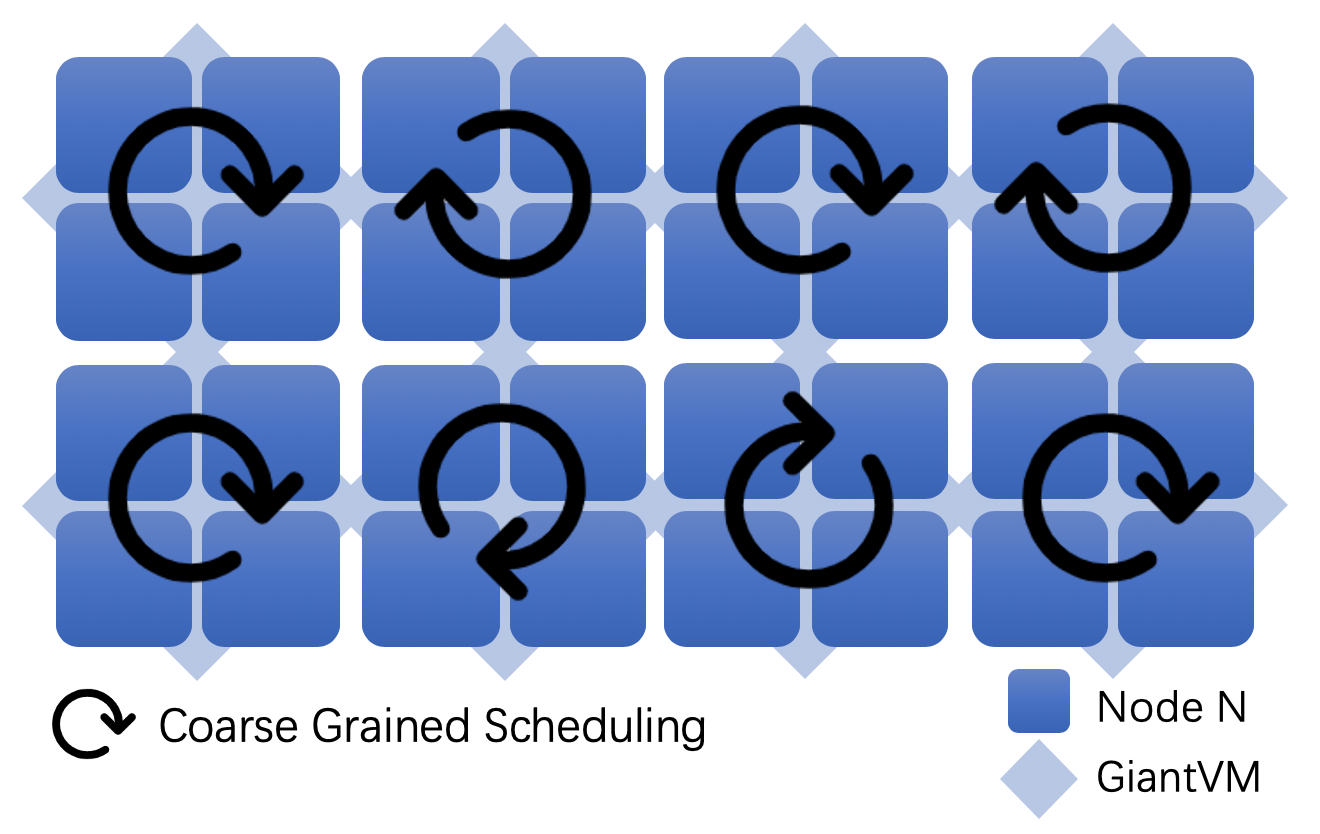
\includegraphics[width=8cm]{coarseschedule.png}
  \bicaption[粗粒度调度器的仿真]
    {粗粒度调度器的仿真}
    {Simulation of Coarse-Grained Scheduler}
  \label{fig:simucoarse}
\end{figure}
我们通过设计调度算法来仿真真实环境下巨型虚拟机中shell脚本的功效。如图\ref{fig:simucoarse}所示,集群中每四个节点部署一个巨型虚拟机,这四个节点组成一个$G\_cell$(GiantVM Cell),每次选取负载最低的一个节点作为进程迁移的目的节点。在我们的实现中,$G\_cell$由四个节点组成,每10个时间戳为一个平衡周期,$migrate()$函数在平衡周期的第一个时间戳被调用。其主要算法类似于算法\ref{algo:coarse}但又有所不同:算法\ref{algo:simucoarse}实现了模拟的粗粒度调度器,$migrate()$函数遍历集群中所有的$G\_cell$,在每个$G\_cell$中,找出负载最低的节点,并且$get\_migratable\_tasks()$函数将$G\_cell$中其余三个节点的可迁移进程保存在$removed$集合中。$get\_migratable\_tasks()$函数判断task是否是可迁移进程的标准是其priority小于2且CPU的最大使用率为0.025以下。接下来,统计该节点所有可迁移进程的资源占用量$util\_diff$。将$util\_diff$加到占用最低的节点上,$is\_useful\_migrate()$函数规定出现以下情况时不可迁移:(1)迁移后占用最低节点的占用率比当前节点高;(2)$util\_diff$大于当前节点负载的80\%;(3)迁移后占用最低节点的占用率超过了节点负载量警戒线(目前设置为节点的最大负载能力,$warning\_threshold$)。如果不符合迁移的条件,则该节点上的可迁移进程不被迁移,并在当前$G\_cell$中继续遍历下一个节点。如果符合迁移条件,$removed$集合中的所有进程将被迁移到$G\_cell$内部负载最低的节点上,同时将这次迁移的网络开销加到$bandwidth\_usage$变量上。对于不开启GiantVM平衡功能的集群,$bandwidth\_usage$将为0,远低于开启GiantVM迁移功能的集群,故GiantVM的迁移也可视作牺牲网络带宽来换取CPU使用率的一种方法。

\begin{algorithm}[h]
\begin{algorithmic}[1]
\Function {migrate}{$timestamp$}
\For{each $G\_cell \in Cluster$}
\State $lowest\_loaded\_node \gets find\_lowest\_loaded\_node(G\_cell,\, timestamp)$
\For{each $node \in (G\_cell - lowest\_loaded\_node)$}
\State $util\_diff,\, removed \gets get\_migratable\_tasks(node,\, timestamp)$
\If{$is\_useful\_migrate(util\_diff,\, removed)$}
\State $bandwidth\_usage \gets bandwidth\_usage + migrate\_to\_node(removed)$
\EndIf
\EndFor
\EndFor
\end{algorithmic}
\caption{粗粒度调度器的仿真算法}
\label{algo:simucoarse}
\end{algorithm}

根据第二章和第三章的分析,粗粒度的调度有助于集群的负载均衡,提高了整体的CPU使用率,且被迁移进程之间不会共享内存。同时,任务的$duration$和机器的$overcommit$都应该下降,因为此调度算法缓解了任务分布不合理所造成的QoS violation,即缓解了单个节点上的CPU需求会短时间爆发性的增长、超过该机器的容载能力的情况,而通过资源重分配利用了长时间处于较低负载状态的机器上多余的资源。仿真算法中,宿主机上的进程可以直接被移送到GiantVM中,被调度到其他节点上,而真实环境下虚拟机和宿主机之间不可以交换进程,这个限制尚未在仿真脚本中进行模拟。事实上,客户机和宿主机之间可以进行网络通信,可以通过网络在客户机与宿主机之间交换进程,这一方案的可行性尚未调查。

\section{细粒度调度器的仿真与调优}
上节所述的粗粒度调度器存在许多可以优化的方面:粗粒度调度器只在$G\_cell$中选取负载最低的节点($lowest\_loaded\_node$),事实上$G\_cell$中可能存在和$lowest\_loaded\_node$负载状况相近的节点,这些负载同样很低的节点没有得到充分利用;其次,粗粒度调度器中对除了$lowest\_loaded\_node$之外的所有节点的任务进行筛选,选出可以迁移的优先级较低的任务迁移到$lowest\_loaded\_node$上。这样会造成较大的网络开销,例如$G\_cell$中有四个节点,则需要将三个节点上的可迁移进程全部进行迁移。这个问题在真实环境下也存在:真实环境下的巨型虚拟机调度器将客户机中所有的进程在NUMA节点之间迁移,而整个操作系统中的进程内存总量是很可观的,从而也会造成单节点上的网络带宽被严重占用。

\subsection{细粒度调度器的仿真}
\begin{figure}[!htp]
  \centering
  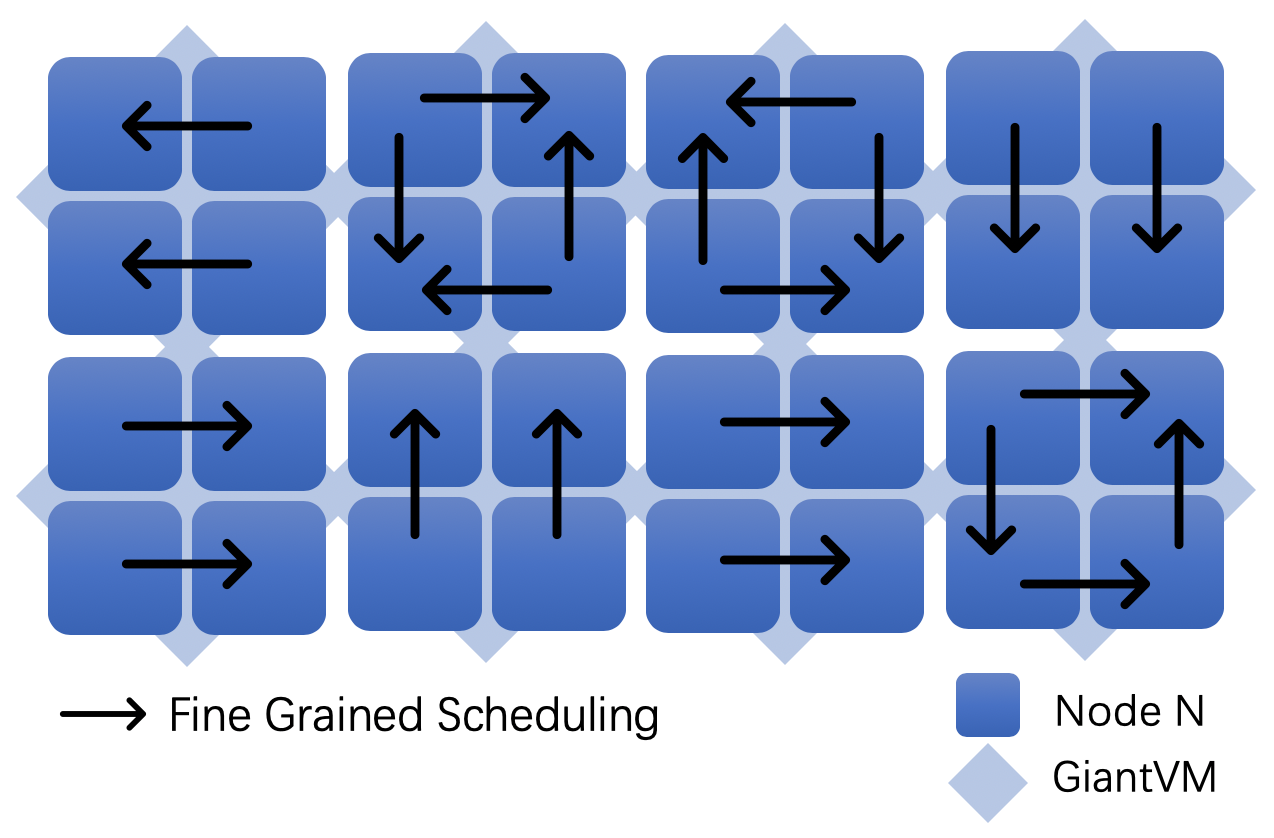
\includegraphics[width=8cm]{fineschedule.png}
  \bicaption[细粒度调度器的仿真]
    {细粒度调度器的仿真}
    {Simulation of Fine-Grained Scheduler}
  \label{fig:simufine}
\end{figure}
为了解决粗粒度调度器所遇到的性能问题,我们设计了细粒度的调度器。算法\ref{algo:simufine}说明了该调度算法的大致过程:和粗粒度的调度算法一样,细粒度算法遍历集群中所有的$G\_cell$,而与粗粒度算法不同的是,我们在一个$G\_cell$中找出负载最低的两个节点,而其他节点遍历其所有进程,找出可迁移进程,加入到$removed$集合中。相对于粗粒度的调度算法,我们认为细粒度的调度算法有较小的网络开销,由于在网络之中迁移的$removed$集合更少。假如一个$G\_cell$中有四个节点,则每个迁移周期中被网络传输的只有两个$removed$集合,而粗粒度的调度算法需要迁移三个$removed$集合。找出节点的$removed$集合后,首先向负载最低的节点迁移$removed$集合中的进程,直到负载最低的节点无法接收新的进程,接下来向负载第二低的节点迁移迁移$removed$集合中的进程,直到第二低负载节点无法接收新的进程。节点是否能接收新进程的判断标准与粗粒度的算法相同,即进程迁移的目的节点的负载不能大于源节点的负载,也不能大于负载警戒线$warning\_threshold$。当负载最低节点和负载第二低节点的接收列表$move\_to\_first$、$move\_to\_second$被填满后,统计两个列表的任务的CPU使用量,当使用量超过一定的阈值才可进行真正的迁移(由$is\_useful\_migrate()$函数判断)。
\begin{algorithm}[h]
\begin{algorithmic}[1]
\Function {migrate}{$timestamp$}
\For{each $G\_cell \in Cluster$}
\State $lowest\_loaded\_node,\,second\_lowest\_loaded\_node \gets find\_lowests(G\_cell,\, timestamp)$
\For{each $node \in (G\_cell - lowest\_loaded\_node - second\_lowest\_loaded\_node)$}
\State $removed \gets get\_migratable\_tasks(node,\, timestamp)$
\While{$first\_lowest\_can\_hold(timestamp)\,and\,!remove.empty()$}
\State $move\_to\_first.add(removed.pop())$
\EndWhile
\While{$second\_lowest\_can\_hold(timestamp)\,and\,!remove.empty()$}
\State $move\_to\_second.add(removed.pop())$
\EndWhile
\If{$is\_useful\_migrate(util(move\_to\_first))$}
\State $bandwidth\_usage \gets bandwidth\_usage + migrate\_to\_first(move\_to\_first)$
\EndIf
\If{$is\_useful\_migrate(util(move\_to\_second)$}
\State $bandwidth\_usage \gets bandwidth\_usage + migrate\_to\_second(move\_to\_second)$
\EndIf
\EndFor
\EndFor
\end{algorithmic}
\caption{细粒度调度器的仿真算法}
\label{algo:simufine}
\end{algorithm}

如图\ref{fig:simufine}所示,细粒度的调度算法发生在两组节点之间。举例而言,对于$G\_cell$大小为4的集群,节点编号为node0-3,假设负载情况是node0\,<\,node1\,<\,node2\,<\,node3,那么进程将会由node2,3向node0,1迁移。而对比粗粒度的调度算法,只有node0作为接收进程的节点,需要同时接收来自于node1-3的可迁移进程。假设所有的节点不存在无法接收被迁移进程的情况(即资源充足),那么node0将会接收3个$removed$集合的进程,不但对node0的网络带宽造成较大压力,也使得node0的CPU负载迅速升高,但其他节点的CPU使用率一律降低,造成了CPU使用率的不均衡。而对于细粒度调度算法,node0,1平均只需接收来自于一个节点的$removed$集合,网络开销明显减小,且node0,1分担了CPU负载,CPU负载不会大幅度上升。所以我们认为,细粒度的调度算法具有更强的集群负载平衡能力,也具有较小的网络开销。

\subsection{排序的细粒度调度算法}
在众多的调度器中,排序是提高调度器效率的重要方法,例如Linux\cite{linux}的完全公平调度器使用红黑树将进程按照$vruntime$排序,使得进程公平地拥有运行时间。在巨型虚拟机的调度算法中,依然可以应用排序。根据谷歌提供的集群追踪数据,我们有两种排序的方案:

\noindent\textbf{根据CPU数据排序}\quad 谷歌的集群追踪数据中可用于CPU使用情况排序的数据有:$task\_usage$表中的进程每个时刻的CPU使用率$Task.usage[cpu]$,以及$task\_event$表中进程CPU使用率上限$Task.request$。我们认为,将CPU使用率较低的进程优先调度有助于提高集群的CPU使用率。举例而言,假设最低的节点剩余的CPU负载能力为1,而可供迁移的进程的CPU使用量是0.6,0.45,0.43。如果按照CPU使用率高的进程优先调度,则被迁移到负载最低节点上的进程为0.6,还剩余0.4未占用的CPU负载能力;如果按照CPU使用率低的进程优先调度,则进程0.45,0.43被调度,占用了0.87的空闲CPU,高于按照CPU使用率高的优先调度的情况。这是因为CPU使用率高的进程会在空余的CPU负载能力中造成较大的碎片,例如在这个例子中,0.6的进程造成了0.4的碎片,是空闲CPU使用量的40\%。事实上,向空余CPU中填充进程的问题是一个背包问题,即:背包可以容纳重量为1的物品,每件物品的价值和重量相等,分别为0.6,0.45,0.43。背包问题一个NP完全问题,本文优先调度CPU占用较低的进程,用贪心法求得近似解。对于表征CPU使用量的数据选取,我们认为$Task.usage[cpu]$比$Task.request$更具有代表性,因为$Task.usage$是实时获取的数据,更有利于动态计算集群中的任务负载情况。

\noindent\textbf{根据内存数据排序}\quad 对内存使用情况进行排序的主要目的是降低网络的开销。我们使用的谷歌的集群追踪数据主要提供了进程的两个内存使用情况的数据:$Task.usage[memory]$每个时刻下进程容器所使用的总的内存页数量,称作assigned memory,包含该任务的用户态和内核态页面,也是谷歌Borg集群中容器迁移所要迁移的真正的页面数量(见\ref{chap:containermigration}节的背景介绍);$Task.usage[MPI]$,平均每条指令的访存次数(memory accesses per instruction),通过performance counter获得\footnote{performance counter\cite{perf}是CPU硬件上的一组寄存器,记录了各类硬件事件,包括分支预测错误、缓存不命中次数、指令执行次数等。}。一个进程所拥有的内存页的数量与缓存不命中的频率有一些关系,但关联性不是很强:CPU密集型任务拥有的内存页较少,MPI也较低;内存密集型任务的MPI较高,但其经常访问的内存页的数目不一定大,也存在拥有大量内存页的进程的MPI较低的情况,故MPI反映了进程频繁访问内存页面的数量。如果优先调度内存占用$Task.usage[memory]$高的进程,将会有效地减小迁移的网络开销。由于细粒度的调度器将可调度进程分为两组(在真实情况下,巨型虚拟机的任务将在两个NUMA节点上运行),这两组进程可能会产生大量的共享内存访问(见\ref{chap:memm}节)。但是由于谷歌的追踪数据未提供进程访问内存的具体位置,所以我们无法对此情况进行仿真。

排序的细粒度调度算法由算法\ref{algo:sorted}表述。我们提供了6个$option$,作为测试比较的对象,分别为:

\begin{itemize}
  \item 0:不排序;
  \item 1:按照进程的CPU使用率上限(CPU request)从小到大排序;
  \item 2:按照$timestamp$时刻的CPU使用量从小到大排序
  \item 3:按照$timestamp$时刻的内存使用量从小到大排序
  \item 4:按照$timestamp$时刻的CPU使用量从大到小排序
  \item 5:按照$timestamp$时刻的MPI从小到大排序
\end{itemize}

\begin{algorithm}[h]
\begin{algorithmic}[1]
\Function {migrate}{$timestamp$}
\State $...... /* Same \,as\, algorithm\,$\ref{algo:simufine}$\,*/$
\State $removed \gets get\_migratable\_tasks(node,\, timestamp)$
\State $option \gets get\_option()$
\State $sort\_tasks(option,\,removed)$
\State $...... /* Same \,as\, algorithm\,$\ref{algo:simufine}$\,*/$
\end{algorithmic}
\caption{排序的细粒度调度器}
\label{algo:sorted}
\end{algorithm}

\section{本章小结}
本章通过仿真一个具有800个相同机器的集群,通过python脚本实现了便利、快捷且有效的仿真条件,模拟了第三章真实环境下的巨型虚拟机平衡调度器。分析了粗粒度调度器存在的性能问题,如网络开销太大、集群资源利用率仍不平衡,并设计了细粒度的进程调度器。分析了进程调度顺序对平衡效果以及网络开销的影响,设计了排序的细粒度调度器,并且提供了6种不同的排序选项。我们将在下一章对这6个排序选项进行性能测试和分析。